%!TEX root = ../thesis.tex
\section{緒言}
本章では3章で実装した歩行パターン生成器を用いて,実際に歩行パターンを生成した結果を示す.
\section{実験の設定}
本研究で開発したソフトウェアを使用し,表\ref{tb:parametor}に示すパラメータで重心とZMPの軌道を3000[ms]の長さに渡って生成した.ここで,制約はソフト制約とする.

\begin{table}[htbp]
  \centering
  \begin{tabular}{|c|c|} \hline
    Control Horizon & 1.5 [$s$] \\ \hline
    Unit time &10 [$ms$] \\ \hline
    Q / R  & 100000.0 \\ \hline
    Height of CoM & 0.6 [$m$] \\ \hline
    Step width & 0.15 [$m$] \\ \hline
    Upper bound of difference between ref and current output. & 0.02 [$m$] \\ \hline
    Lower bound of difference between ref and current output. & -0.02 [$m$] \\ \hline
    Upper bound of input & 100 [$m/s^{3}$] \\ \hline
    Lower bound of input & -100 [$m/s^{3}$] \\ \hline
  \end{tabular}
  \caption{Libraries used for implementation}
  \label{tb:parametor}
\end{table}

\newpage

次に,生成した重心とZMPの軌道,最適入力を図\ref{Fig:zmptrajectory}と図\ref{Fig:optimalinput}に示す.

\begin{figure}[hbtp]
  \centering
 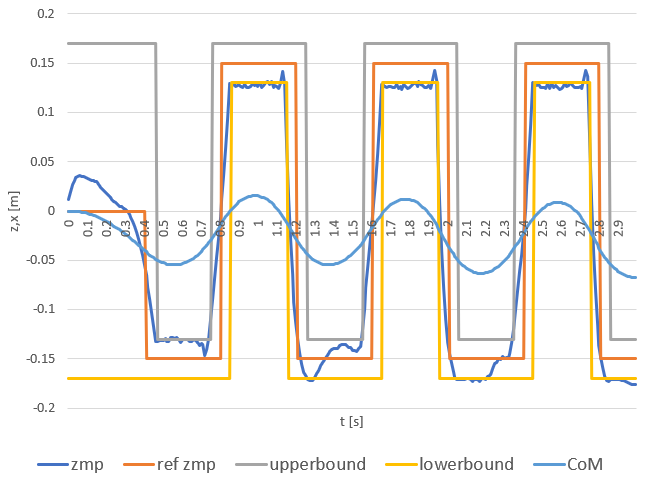
\includegraphics[keepaspectratio, scale=0.6]
      {images/zmp_trajectory.png}
 \caption{Generated zmp and CoM trajectory }
 \label{Fig:zmptrajectory}
\end{figure}

\begin{figure}[hbtp]
  \centering
 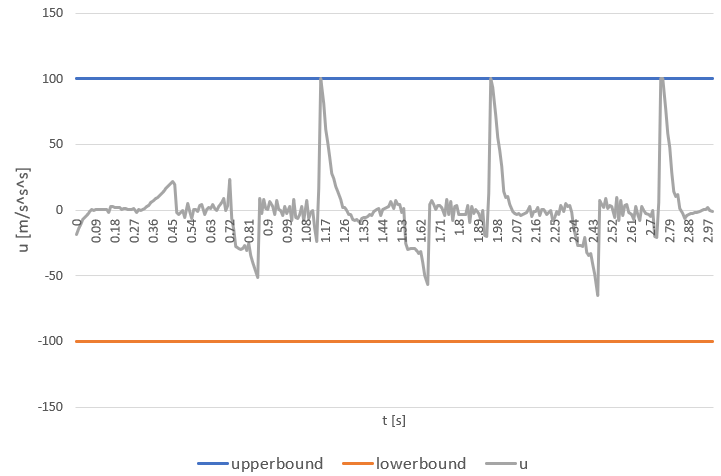
\includegraphics[keepaspectratio, scale=0.6]
      {images/calculated_input.png}
\caption{Optimal input}
 \label{Fig:optimalinput}
\end{figure}

\newpage
図\ref{Fig:zmptrajectory} より,ZMP が目標 ZMP に追従する軌道が生成できていることが分かる. また,図\ref{Fig:zmptrajectory}より状態が ,図\ref{Fig:optimalinput}より入力が設定した制約の範囲に対して致命的な違反を起こしておらず,適切な歩行パターンが生成できていることも分かる.


